% -- Encoding UTF-8 without BOM
% -- XeLaTeX => PDF (BIBER)

\documentclass{cv-style}     % Add 'print' as an option into the square bracket to remove colours from this template for printing. 
                                      % Add 'espanol' as an option into the square bracket to change the date format of the Last Updated Text
%\setdefaultlanguage{spanish}
%\sethyphenation[variant=spanish]{}{}  % Add words between the {} to avoid them to be cut 

\usepackage{graphicx}


\begin{document}


\header{Nathan}{Mitchell}
\lastupdated

%----------------------------------------------------------------------------------------
% SIDEBAR SECTION  -- In the aside, each new line forces a line break
%----------------------------------------------------------------------------------------
\begin{aside}
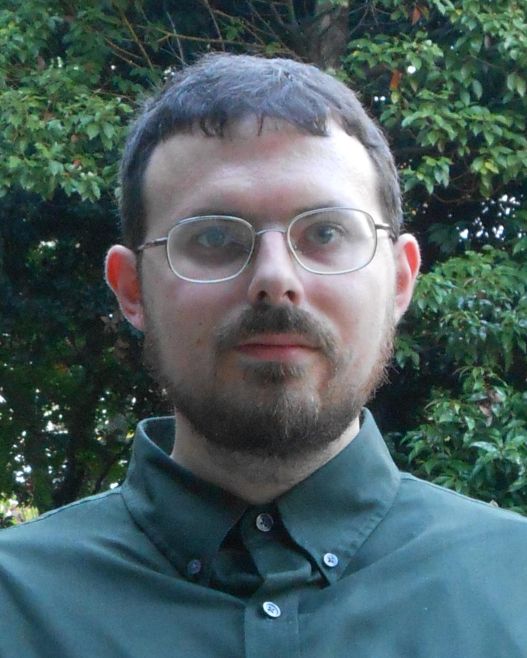
\includegraphics[width=4cm]{NMitchell_Portrait}
%
\section{Personal Information}
Nathan Mitchell
B.S, M.S. Computer Science
http://nathanmitchell.graphics
\section{Contact}
Email (Preferred):
{\footnotesize \bf contact@nathanmitchell.graphics}
Tel:
(608) 509-4176
\section{Programming Languages}
\textbf{C++}, \textbf{C}, \textbf{Python}, x86 Assembly, Bash/Zsh Scripting,
Java, Cobol
%
\section{Tools}
Electron, LaTeX, Blender, Renderman, Adobe
Illustrator, Adobe Premiere, Intel VTune
\section{Miscellaneous Technologies}
Ubuntu/Debian, RabbitMQ,
Git/Mercurial Version
Control, SQL, NodeJS, OpenGL
%
\end{aside}
%----------------------------------------------------------------------------------------
% RESUMEN SECTION
%----------------------------------------------------------------------------------------
\vspace{0.2cm}
\section{R\'{e}sum\'{e}}
\vspace{-0.2cm} My name is Nathan Mitchell and I
am a finishing PhD student at the University of
Wisconsin - Madison and a member of the UW Visual
Computing Lab. My primary academic interests
include physics simulation for deformable objects,
software optimization for heterogeneous hardware,
and rendering. I enjoy working on large software
systems, particularly in the design of elegant
APIs for long term maintainability.

My advisor at the University of Wisconsin is Dr. Eftychios Sifakis. Before
I began my graduate program, I attended the University of Edinboro in
Pennsylvania for my undergraduate degree in computer science. I have
also worked with the Math and Computer Science division of Argonne
National Labs, where I helped develop software for managing cluster
provisioning.

%----------------------------------------------------------------------------------------
% EDUCATION SECTION
%----------------------------------------------------------------------------------------
\section{Education}
  \vspace{-0.2cm}
\begin{entrylist}
%------------------------------------------------
\entry
{\scalebox{.8}[1.0]{2013--Today}}
{PhD. Computer Sciences}
{University of Wisconsin - Madison}
{(est. completion: May. 2017)}
%------------------------------------------------
\entry
{\scalebox{.8}[1.0]{2010--2013}}
{Masters of Computer Sciences}
{University of Wisconsin - Madison}
{}
%------------------------------------------------
\entry
{\scalebox{.8}[1.0]{2005--2009}}
{Bachelors of Computer Science}
{University of Edinboro}
{}
%------------------------------------------------
\end{entrylist}
%----------------------------------------------------------------------------------------
% AWARDS SECTION
%----------------------------------------------------------------------------------------
  \vspace{-0.2cm}
\section{Publications}
  \vspace{-0.2cm}
\begin{entrylist}
%------------------------------------------------
\entry
{\scalebox{.8}[1.0]{2017}}
{}
{In Submission}
{\textit{H. Liu, N. Mitchell, M. Aanjaneya, J. Lowe-Power, M. Aanjaneya, E. Sifakis} \textbf{A Hierarchical Domain Decomposition Preconditioner for the Poisson Equation Optimized for Heterogeneous Platforms}  in proceedings of
Supercomputing, 2017}
%------------------------------------------------
\end{entrylist}
\begin{entrylist}
\entry
{\scalebox{.8}[1.0]{2016}}
{}
{Presented at SIGGRAPH Asia 2016}
{\textit{H. Liu, N. Mitchell, M. Aanjaneya, E. Sifakis} \textbf{A
scalable Schur-complement fluids solver for
heterogeneous compute platforms}  in proceedings of
ACM SIGGRAPH Asia, 2016}
%------------------------------------------------
\entry
{\scalebox{.8}[1.0]{}}
{}
{}
{\textit{N. Mitchell, C. Cutting, T. King, A. Oliker,
E. Sifakis}  \textbf{A Real-Time Local Flaps Surgical
Simulator Based on Advances in Computational
Algorithms for Finite Element Models}  Plastic \&
Reconstructive Surgery. 137(2):445e-452e, February
2016., 2016}
%------------------------------------------------
\entry
{\scalebox{.8}[1.0]{}}
{}
{Presented at SCA 2016}
{\textit{N. Mitchell, M. Doescher, E. Sifakis}  \textbf{A Macroblock
Optimization for Grid-Based Nonlinear Elasticity}
Eurographics/ACM SIGGRAPH Symposium on Computer
Animation, 2016}
%------------------------------------------------
\end{entrylist}
\begin{entrylist}
\entry
{\scalebox{.8}[1.0]{2015}}
{}
{Presented at SIGGRAPH 2015}
{\textit{N. Mitchell, C. Cutting, E. Sifakis}  \textbf{GRIDiron: An
Interactive Authoring and Cognitive Training
Foundation for Reconstructive Plastic Surgery
Procedures}  in proceedings of ACM SIGGRAPH, 2015}
%------------------------------------------------
\entry
{\scalebox{.8}[1.0]{}}
{}
{Presented at SIGGRAPH Asia 2015}
{\textit{N. Mitchell, M. Aanjaneya, R. Setaluri, E. Sifakis}
\textbf{Non-manifold Level Sets: A multivalued implicit
surface representation with applications to
self-collision processing}  in proceedings of ACM
SIGGRAPH Asia, 2015}
%------------------------------------------------
\end{entrylist}
\begin{entrylist}
\entry
{\scalebox{.8}[1.0]{2014}}
{}
{Presented at SCA 2014}
{\textit{R. Setaluri, Y. Wang, N. Mitchell, L. Kavan,
E. Sifakis}  \textbf{Fast Grid-Based Nonlinear Elasticity
for 2D Deformations}  Eurographics/ACM SIGGRAPH
Symposium on Computer Animation, 2014}
%------------------------------------------------
\entry
{\scalebox{.8}[1.0]{}}
{}
{Presented at SCA 2014}
{\textit{M. Gao, N. Mitchell, E. Sifakis}  \textbf{Steklov-Poincar\'{e}
Skinning}  Eurographics/ACM SIGGRAPH Symposium on
Computer Animation, 2014}
%------------------------------------------------
\end{entrylist}
\begin{entrylist}
\entry
{\scalebox{.8}[1.0]{2012}}
{}
{Presented at SIGGRAPH Asia 2012}
{\textit{T. Patterson, N. Mitchell, E. Sifakis}  \textbf{Simulation
of Complex Nonlinear Elastic Bodies using Lattice
Deformers}  in proceedings of ACM SIGGRAPH Asia,
2012}
%------------------------------------------------
\end{entrylist}
  \vspace{-0.2cm}
%----------------------------------------------------------------------------------------
% WORK EXPERIENCE SECTION
%----------------------------------------------------------------------------------------
\section{Experience}
  \vspace{-0.2cm}
\begin{entrylist}
%------------------------------------------------
\entry
  {\scalebox{.8}[1.0]{2012--Today}}
  {University of Wisconsin - Madison}
  {Madison, Wisconsin - USA}
  {\jobtitle{Research Assistant}\\    
    For the past several years, I have been the
    lead developer on a virtual surgery project,
    which aims to provide a virtual authoring and
    practice tool for plastic surgeons. 
}
%------------------------------------------ ------
%\vspace{-0.3cm}
 \entry
{\scalebox{.8}[1.0]{2008-2010}}
{Argonne National  Laboratory}
{Lemont, Illinois - USA}
{\jobtitle{Intern}\\
  I spent three summers developing management
  software for the Mathematics and Computer
  Science Group at Argonne National
  Laboratory. The first software package was a web
  form deployment system to assist the help desk
  support staff. The second project, named
  \textbf{Heckle}, was a cluster hardware
  provisioning system designed to provide
  on-demand operating system installations
  tailored to user requirements.
  }
%------------------------------------------ ------
%\vspace{-0.3cm}
 \entry
{\scalebox{.8}[1.0]{2005-2006}}
 {Intel}
 {Hillsboro, Oregon - USA}
{\jobtitle{Intern - Technician}\\
 For two summers I worked in the Intel's Hillsboro
 fabrication plant as a manufacturing technician
 for their 200mm production line. The experience
 provided me first hand insight into modern
 integrated circuit manufacturing processes. 
  }

%------------------------------------------------
\end{entrylist}

%----------------------------------------------------------------------------------------
% INTERESTS SECTION
%----------------------------------------------------------------------------------------3
\section{Research Interests}
  \vspace{-0.2cm}

  \textbf{Simulation} I am very interested in
  pursuing further work regarding the pairing of
  bio-medical topics and real-time simulation,
  particularly in the areas of deformable solids
  and plastic surgery. I consider my work at
  Wisconsin to be a solid first step, but with a
  large potential for future work.

  \textbf{Parallel Computing} While there have
  been many different approaches taken over the
  years to make parallel computing easier for
  programmers to make use of, my experience has
  shown that there are still many hurdles to
  overcome, especially in the areas of hardware
  vectorization and optimal use of memory
  bandwidth on highly parallel heterogeneous
  systems. I remain interested in pursing new
  frameworks and design patterns for improving
  a programmer's quality of life when dealing with
  these problems.

  \textbf{Framework Design} Designing and building
  system frameworks, while not typically
  considered glamorous from a academic research
  perspective, is something that I feel is
  critical to designing useful software. I have
  spent a great deal of effort during my prior
  projects to build maintainable and reusable
  components, which have paid dividends in later
  research efforts.

  \textbf{Rendering} My experience here is mostly
  due to the needs of presenting the results of
  high resolution simulations through
  publications. However, the challenges in this area
  have caught my attention and I have a continued
  interest in how highly complex simulated scenes
  can still be rendered efficiently.

  \textbf{Game Design} I have a fascination with
  game mechanics and how interesting design
  choices make for engaging entertainment for
  players. While recently my medium has been
  boardgames, I believe many aspects of good game
  design are shared between the physical and
  electronic realms.

%----------------------------------------------------------------------------------------
% PROJECTS SECTION
%----------------------------------------------------------------------------------------3
%\begin{OptSection}[enable=true,title=Projects]
\section{Projects}
\vspace{-0.2cm}

\textbf{Plastic Surgery Simulation} For the past five years, I have
been developing a simulation system for performing plastic surgery
operations virtually in a collaborative environment. Over the course
of the project, I developed a new SIMD abstraction library for
efficiently optimizing finite element numerical kernels, a novel
strategy for storing level set geometry in non-manifold topology, and
explored approaches for remote simulation, including using modern web
technologies as front-end clients. My efforts, beyond the production
of the software artifacts, resulted in five publications, local news
coverage, and a currently active exploration of commercialization
opportunities.

\textbf{Heckle} During the spring and summer of 2010, I was the lead
developer for a cluster provisioning system named Heckle for Argonne
National Laboratories. Heckle was designed to manage a collection of
potentially heterogeneous compute nodes. The problem being addressed
was that researchers often needed custom hardware (specific CPU,
memory capacity, accelerator cards) for their projects, but didn't
need it long enough to warrant a dedicated machine. Heckle provided users with a single
point of access to request nodes matching specific requirements and
dynamically provision the nodes with custom operating system
images. By interacting with out-of-band management services, Heckle
could remotely power cycle nodes and initiate re-installations without
administrator intervention.

%\end{OptSection}


%----------------------------------------------------------------------------------------
% References SECTION
%----------------------------------------------------------------------------------------3
\section{References}
  \vspace{-0.2cm}

\begin{entrylist}


 \entry
{\scalebox{.8}[1.0]{PhD. Advisor}}
 {Eftychios Sifakis, PhD}
 {Madison, WI - USA}
{
 University of Wisconsin Madison\\
Email : sifakis@cs.wisc.edu\\
URL: http://pages.cs.wisc.edu/\textasciitilde{}sifakis
 } 

 \entry
{\scalebox{.8}[1.0]{PhD. Committee}}
 {Court Cutting, MD}
 {Santa Barbara, CA - USA}
{
Email : ccuttingmd@gmail.com\\
URL: http://www.courtcuttingmd.com
 } 


 \entry
{\scalebox{.8}[1.0]{PhD. Committee}}
 {Mike Gleicher, PhD}
 {Madison, WI - USA}
{
 University of Wisconsin Madison\\
Email : gleicher@cs.wisc.edu\\
URL: http://pages.cs.wisc.edu/\textasciitilde{}gleicher
 } 




\end{entrylist}
%----------------------------------------------------------------------------------------
\end{document}












